\documentclass[a4paper,10pt]{article}%
\input{commands.tex}%

\author{Peter Bonventre, Lu\'is A. Pereira}%
\title{Genuine equivariant operads}%

\usepackage{showkeys}%

\usepackage{stmaryrd}

\usepackage{geometry}

\usepackage{tikz}%
\tikzset{%
  treenode/.style = {shape=rectangle, rounded corners,%
                     draw, align=center,%
                     top color=white, bottom color=blue!20},%
  root/.style     = {treenode, font=\Large, bottom color=red!30},%
  env/.style      = {treenode, font=\ttfamily\normalsize},%
  dummy/.style    = {circle,draw,inner sep=0pt,minimum size=2mm}%
}%

\usetikzlibrary[decorations.pathreplacing]

\begin{document}	\maketitle%


\abstract{We build new algebraic structures, which we call genuine equivariant operads, which can be thought of as a hybrid between equivariant operads and coefficient systems.
We then prove an Elmendorf type theorem stating that equivariant operads, with their graph model structure, are equivalent to genuine equivariant operads with their projective model structure.

As an application, we build explicit models for the $N_{\infty}$-operads of Blumberg and Hill.
}

\tableofcontents

\section{Introduction}

No content yet.



\section{Planar and tall maps}

\subsection{Planar structures}


Throughout we will work with trees possessing \textit{planar structures} or, more intuitively, trees embedded into the plane.

Our preferred model for trees will be that of broad posets first introduced by Weiss in \cite{We12} and further worked out by the second author in \cite{Pe16b}. We now define planar structures in this context.


\begin{definition}\label{PLANARIZE DEF}
	Let $T \in \Omega$ be a tree. A \textit{planar structure} of $T$ is an extension of the descendancy partial order $\leq_d$ to a total order $\leq_p$ such that: 
	\begin{itemize}
		\item \textit{Planar}: if $e \leq_p f$ and $e \nleq_d f$ then 
		$g \leq_d f$ implies $e \leq_p g$.
	\end{itemize} 
\end{definition}


\begin{example}
An example of a planar structure on a tree $T$ follows, with $\leq_r$ encoded by the number labels.
\[
	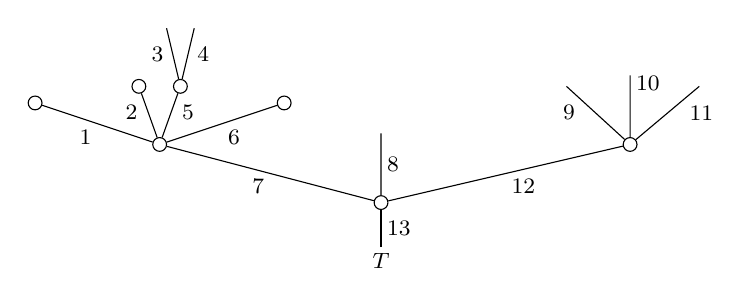
\begin{tikzpicture}[grow=up,auto,level distance=2.1em,
	every node/.style = {font=\footnotesize,inner sep=2pt},
	dummy/.style={circle,draw,inner sep=0pt,minimum size=1.75mm}]
		\node at (0,0) {$T$}
			child{node [dummy] {}
				child[sibling distance = 9em]{node [dummy] {}
					child[sibling distance = 2.5em]{
					edge from parent node [near end,swap] {$11$}}
					child[level distance=2.5em]{
					edge from parent node [very near end,swap] {$10$}}				
					child[sibling distance = 2.3em]{
					edge from parent node [near end] {$9$}}
				edge from parent node [swap] {12}}
				child[level distance =2.5em]{
				edge from parent node [swap] {$8$}}
				child[sibling distance = 8em]{node [dummy] {}
					child[sibling distance =3em, level distance = 1.5 em]{node [dummy] {}
					edge from parent node [swap] {$6$}}
					child[sibling distance = 1.5em]{node [dummy] {}
						child[sibling distance =1em]{
						edge from parent node [swap,near end] {$4$}}
						child[sibling distance =1em]{
						edge from parent node [near end] {$3$}}
					edge from parent node [very near end,swap] {$5$}}
					child[sibling distance =1.5em]{node [dummy] {}
					edge from parent node [very near end] {$2$}}
					child[sibling distance =3em,level distance =1.5em]{node [dummy] {}
					edge from parent node {$1$}}
				edge from parent node {$7$}}
			edge from parent node [swap] {$13$}};
	\end{tikzpicture}
\]
Intuitively, given a planar depiction of a tree $T$, $e \leq_d f$ holds when the downward path from $e$ passes through $f$
and $e \leq_p f$ holds if either
$e \leq_d f$ or if the downward path from $e$ is to the left of the downward path from $f$ (as measured by the node where they intersect).


{\color{red} HERE}

a planarization of $T$ encodes the exact same information as a depiction of $T$ in the plane, though we will not  need to make this idea precise. Informally,
 a $e \leq_p f$ relation dictates that either: 
\begin{inparaenum}
	\item [(i)] $e$ appears above $f$, should it be $e \leq_d f$, or; that ``the path from $e$ to the root is to the left of the path from $f$ to the root'', should it be $e \nleq_d f$.
\end{inparaenum}
\end{example}


We now establish some basic properties of planarizations. We start with some notation.


\begin{notation}\label{INPUTPATH NOT}
	Let $T \in \Omega$ be a tree and $e \in T$ and edge. We will denote
	\[ I(e) =\{f \in T \colon e \leq_d f \} \]
and refer to this poset as the \textit{input path of $e$}.
\end{notation}

\begin{notation}
	Let $T \in \Omega$ be a tree and suppose that $e <_d f$. We will denote by $f^{\uparrow}_e \in T$ the only edge $f^{\uparrow}_e \in f^{\uparrow}$ such that 
	$e \leq_f f^{\uparrow}_e$.
\end{notation}


\begin{proposition}
	Let $T \in \Omega$ be a tree. Then
	\begin{itemize}
		\item[(a)] for any $e \in T$ the finite poset $I(e)$ is totally ordered;
		\item[(b)] the edge $g \in I(e)$ is the successor of 
		$f \in I(e)$ iff $f \in g^{\uparrow}$ iff $f=g^{\uparrow}_f$; 
		\item[(c)] the poset $(T,\leq_d)$ has all joins.
	\end{itemize}
\end{proposition}

\begin{proof}
	To prove (a), note that if any two edges in $I(e)$ were $\leq_d$ incomparable, then {\color{green} Eq.D.S. Lemma 4.14} would lead to a non-simple broad relation for the root of $T$.
	(b) follows since $f \leq g^{\uparrow}_f$.

	To prove (c), note that 
	$\min (\bigcap_{i=1}^n I(e_i))$ exists by (a), and this is clearly the join $\bigvee_{i=1}^n{e_i}$.
\end{proof}

\begin{proposition}
\label{TERNARYJOIN PROP}
All ternary joins in $(T,\leq_d)$ are binary, i.e.
\[ e_1 \vee e_2 \vee e_3 = e_i \vee e_j\]
for some $1\leq i <j \leq 3$. Further, $e_1 \vee e_2 \vee e_3 \neq e_i \vee e_j$ can hold for at most one choice of $1\leq i <j \leq 3$.
\end{proposition}

\begin{proof}
By definition of join the edges 
$(e_1 \vee e_2 \vee e_3)^\uparrow_{e_1}$, 
$(e_1 \vee e_2 \vee e_3)^\uparrow_{e_2}$, 
$(e_1 \vee e_2 \vee e_3)^\uparrow_{e_3}$
can not all coincide. Noting that hence at most two of these edges are the same yields the result.
\end{proof}


\begin{proposition}\label{PLANARIZATIONCHAR PROP}
	Let $T \in \Omega$ be a tree. There is a bijection {\color{green}(change $\Sigma$ notation)}
	\begin{equation}\label{PLANAR EQ}
	\begin{tikzcd}[row sep = 0.5em]
		\{\text{planarizations }(T,\leq_p)\} \ar[r] &
		\prod_{(e^{\uparrow} \leq e) \in V(T)} \Sigma_{e^{\uparrow}} \\
		\leq_p \ar[mapsto]{r} & (\leq_p|_{e^{\uparrow}})
	\end{tikzcd}	
	\end{equation}
\end{proposition}

\begin{proof}
	Suppose $e, f$ are $\leq_d$-incomparable edges. One must then have $e,f <_d  e \vee f$ as well as 
	$(e \vee f)^{\uparrow}_e \neq (e \vee f)^{\uparrow}_f$. Without loss of generality, we may assume 
	\begin{equation}\label{PLANARORDERDEF}
		(e \vee f)^{\uparrow}_e <_p (e \vee f)^{\uparrow}_f
	\end{equation}
and the relations 
$e \leq_d (e \vee f)^{\uparrow}_e <_p (e \vee f)^{\uparrow}_f \geq_d f$ now show that $e \leq_p f$, and hence (\ref{PLANAR EQ}) is injective.

To see that (\ref{PLANAR EQ}) is surjective, it suffices to check that for $\leq_d$-incomparable $e,f$, defining $e \leq_p f$ to hold iff 
(\ref{PLANARORDERDEF}) holds yields a planarization. 
In the remainder of the proof, we abuse notation by writing $e<_p f$ to denote (\ref{PLANARORDERDEF}) together with the assumption that $e,f$ are $\leq_d$-incomparable. The antisymmetry and total order conditions are immediate. Now suppose that
\begin{equation}\label{TRANSITIV1 EQ}
	e' \leq_d e \qquad  f' \geq_d f \qquad e \vee f \neq e,f.
\end{equation}
Noting that $e' \vee f'$ must be $\leq_d$-comparable with both $e$ and $f$ (since the relevant pairs lie in either $I(e')$ or $I(f')$), one sees that it must be $e,f <_d  e' \vee f'$ (since otherwise all three would lie in either $I(e')$ or $I(f')$) and that hence
$e \vee f = e' \vee f'$ and 
$(e \vee f)^{\uparrow}_e=(e \vee f)^{\uparrow}_{e'}$, 
$(e \vee f)^{\uparrow}_f=(e \vee f)^{\uparrow}_{f'}$. 
Therefore, in the conditions of (\ref{TRANSITIV1 EQ}) one has 
$e <_p f$ iff $e'<_p f'$. The planar condition and the non-trivial instances of transitivity thus follow, with the single exception of the $e <_p f <_p g$ case. 
To check this last case, note that by Proposition \ref{TERNARYJOIN PROP} either:
\begin{inparaenum}
	\item[(i)] both  
$e \vee f$, $f \vee g$ equal $e \vee f \vee g$, in which case  
 $(e \vee f \vee g)^{\uparrow}_e <_p
(e \vee f \vee g)^{\uparrow}_f <_p
(e \vee f \vee g)^{\uparrow}_g 
 $ 
implies that $e \vee g$ must also equal $e \vee f \vee g$ and transitivity follows;
	\item[(ii)] $e \vee f <_d e \vee f \vee g$, in which case 
	transitivity follows from noting that 
	$(e \vee f \vee g)^{\uparrow}_e = (e \vee f \vee g)^{\uparrow}_f$;
	\item[(iii)] $f \vee g <_d e \vee f \vee g$, which follows just as the previous case.
\end{inparaenum}
\end{proof}

\begin{remark}
	Definition \ref{PLANARIZE DEF} readily extends to forests $F \in \Phi$. The analogue of Proposition \ref{PLANARIZATIONCHAR PROP} then states that the data of a planarization is equivalent to total orderings of the vertices of $F$ together with a total ordering of the roots of $F$. The interested reader may wish to suitably modify the proof of Proposition \ref{PLANARIZE DEF} to obtain this result. Instead, we simply note that planarizations of $F$ are clearly in bijection with planarizations of the join tree $F \star \eta$ (cf. {\color{green} Equiv. dend. sets}).
\end{remark}


\begin{convention}\label{PLANARCONV CON}
	From now on, we will write $\Omega$ (resp. $\Omega_G$) to denote a model for the category of trees (resp. $G$-trees) where
\begin{itemize}	
	\item each object (i.e. tree) is equipped with a planar structure;
	\item morphisms ignore the planar structure;
	\item there is exactly one representative of each planarization, i.e. the identities are the only isomorphisms that preserve the planar structure.
\end{itemize}
\end{convention}

\begin{remark}\label{CONCRETETREE REM}
	The reader desiring extra concreteness is welcome to think of the objects of $\Omega$, $\Omega_G$ as consisting of planarized tree structures on one of the sets 
	$\underline{n} = \{1,2,\cdots,n\}$
such that the planarization $\leq_d$ is the canonical total order. Some trees depicted in this convention follow.
\begin{equation}\label{PLANAROMEGAEX1 EQ}
	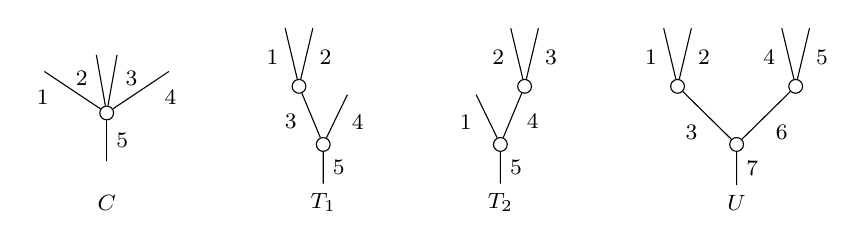
\begin{tikzpicture}[grow=up,auto,level distance=2.1em,every node/.style = {font=\footnotesize},dummy/.style={circle,draw,inner sep=0pt,minimum size=1.75mm}]
		\node at (0,0) {$C$};
		\node at (0,0.4) {}
			child{node [dummy] {}
				child[sibling distance = 1.5em,level distance= 1.5em]{
				edge from parent node [swap,near end] {$4$}}
				child[sibling distance = 0.75em]{
				edge from parent node [swap, very near end] {$3$}}
				child[sibling distance = 0.75em]{
				edge from parent node [very near end] {$2$}}
				child[sibling distance = 1.5em,level distance= 1.5em]{
				edge from parent node [near end] {$1$}}
			edge from parent node [swap] {$5$}};
		\node at (2.75,0) {$T_1$}
			child{node [dummy] {}
				child[sibling distance = 1.75em, level distance=1.8em]{
				edge from parent node[swap, near end] {$4$}}
				child[sibling distance = 1.75em]{node [dummy] {}
					child[sibling distance = 1em]{
					edge from parent node [swap,near end] {$2$}}
					child[sibling distance = 1em]{
					edge from parent node [near end] {$1$}}
				edge from parent node [near end] {$3$}}
			edge from parent node [swap] {$5$}};
		\node at (5,0) {$T_2$}
			child{node [dummy] {}
				child[sibling distance = 1.75em]{node [dummy] {}
					child[sibling distance = 1em]{
					edge from parent node [swap,near end] {$3$}}
					child[sibling distance = 1em]{
					edge from parent node [near end] {$2$}}
				edge from parent node [swap,near end] {$4$}}
				child[sibling distance = 1.75em, level distance=1.8em]{
				edge from parent node[near end] {$1$}}
			edge from parent node [swap] {$5$}};
		\node at  (8,0) {$U$}
			child{node [dummy] {}
				child{node [dummy] {}
					child[sibling distance = 1em]{
					edge from parent node [swap,near end] {$5$}}
					child[sibling distance = 1em]{
					edge from parent node [near end] {$4$}}
				edge from parent node [swap] {$6$}}
				child{node [dummy] {}
					child[sibling distance = 1em]{
					edge from parent node [swap,near end] {$2$}}
					child[sibling distance = 1em]{
					edge from parent node [near end] {$1$}}
				edge from parent node {$3$}}
			edge from parent node [swap] {$7$}};
	\end{tikzpicture}
\end{equation}
\end{remark}
We note that $T_1$ and $T_2$ are isomorphic and, moreover, they encode the only two isomorphism classes of planar structures on the their underlying dendroidal set, so that no other object of $\Omega$ is isomorphic to them. $C$ and $U$, on the other hand, are isomorphic to no other object of $\Omega$, since the  planarizations of the underlying broad posets sets are unique up to isomorphism. 

One drawback of the concrete convention 
illustrated in (\ref{PLANAROMEGAEX1 EQ}), 
however, is that discussion of subfaces of trees becomes awkward, since one can not then technically regard them as subobjects. To avoid this issue, we will often regard the objects of $\Omega$ as equivalence classes of trees with planarizations 
(with no ambiguity resulting since representatives are related via unique isomorphisms).
Moreover, this is particularly convenient when discussing $G$-trees, as it otherwise the task of depicting the $G$-action becomes cumbersome. For some examples, (and recalling that the numbering of the edges as in (\ref{PLANAROMEGAEX1 EQ}) is superfluous, in the sense that it is already encoded in the planar picture itself), we note that for $G=\mathbb{Z}_{/3}$ the orbital representation on the left below encodes the two isomorphic objects of $\Omega_G$ on the right 
(which are isomorphic to no other object of $\Omega_G$).
\[
	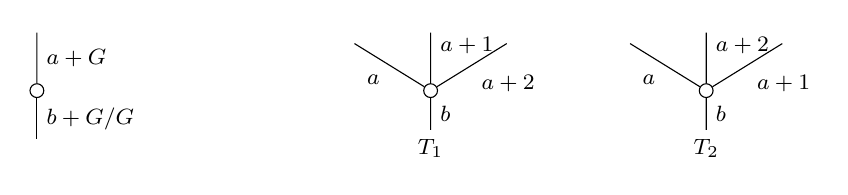
\begin{tikzpicture}[grow=up,auto,level distance=2.1em,every node/.style = {font=\footnotesize},dummy/.style={circle,draw,inner sep=0pt,minimum size=1.75mm}]
		\node at (0,0) {}
			child{node [dummy] {}
				child{
				edge from parent node [swap] {$a+G$}}
			edge from parent node [swap] {$b+G/G$}};
		\node at (5,0) {$T_1$}
			child{node [dummy] {}
				child[level distance=1.7em,sibling distance = 2.75em]{
				edge from parent node [swap] {$a+2$}}
				child{
				edge from parent node [swap, near end] {$a+1$}}
				child[level distance=1.7em,sibling distance = 2.75em]{
				edge from parent node {$a$}}
			edge from parent node [swap] {$b$}};
		\node at (8.5,0) {$T_2$}
			child{node [dummy] {}
				child[level distance=1.7em,sibling distance = 2.75em]{
				edge from parent node [swap] {$a+1$}}
				child{
				edge from parent node [swap, near end] {$a+2$}}
				child[level distance=1.7em,sibling distance = 2.75em]{
				edge from parent node {$a$}}
			edge from parent node [swap] {$b$}};
	\end{tikzpicture}
\]
Similarly, for $G=\mathbb{Z}_{/2}$, the orbital representation on the left represents the two $G$-trees presented.
\[
	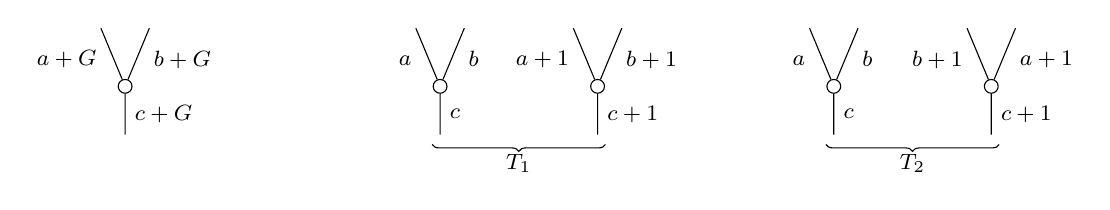
\begin{tikzpicture}[grow=up,auto,level distance=2.1em,every node/.style = {font=\footnotesize},dummy/.style={circle,draw,inner sep=0pt,minimum size=1.75mm}]
		\node at (-1,0) {}
			child{node [dummy] {}
				child[sibling distance=1.75em]{
				edge from parent node [swap,near end] {$b+G$}}
				child[sibling distance=1.75em]{
				edge from parent node [near end]  {$a+G$}}
			edge from parent node [swap] {$c+G$}};
		\node at (3,0) {}
			child{node [dummy] {}
				child[sibling distance=1.75em]{
				edge from parent node [swap,near end] {$b$}}
				child[sibling distance=1.75em]{
				edge from parent node [near end]  {$\phantom{1+}a$}}
			edge from parent node [swap] {$c$}};
		\node at (5,0) {}
			child{node [dummy] {}
				child[sibling distance=1.75em]{
				edge from parent node [swap,near end] {$b+1$}}
				child[sibling distance=1.75em]{
				edge from parent node [near end]  {$a+1$}}
			edge from parent node [swap] {$c+1$}};
		\draw[decorate,decoration={brace,amplitude=2.5pt}] (5.1,0) -- (2.9,0) node[midway]{$T_1$};
		\node at (8,0) {}
			child{node [dummy] {}
				child[sibling distance=1.75em]{
				edge from parent node [swap,near end] {$b$}}
				child[sibling distance=1.75em]{
				edge from parent node [near end]  {$\phantom{1+}a$}}
			edge from parent node [swap] {$c$}};
		\node at (10,0) {}
			child{node [dummy] {}
				child[sibling distance=1.75em]{
				edge from parent node [swap,near end] {$a+1$}}
				child[sibling distance=1.75em]{
				edge from parent node [near end]  {$b+1$}}
			edge from parent node [swap] {$c+1$}};
		\draw[decorate,decoration={brace,amplitude=2.5pt}] (10.1,0) -- (7.9,0) node[midway]{$T_2$};
	\end{tikzpicture}
\]



\bibliography{biblio}{}



\bibliographystyle{abbrv}



\end{document}